Conceptualmente, el modelo de datos del sistema Thary utiliza un modelo relacional, en el que la informacion se organiza en 12 tablas relacionadas entre si, definidas mediante claves foraneas: empresas, usuarios, pedidos, actividad (el historial de movimientos), y corridas. Esta ultima es la tabla principal que representa cada vez que un usuario (administrador) sube un CSV, junto con 7 tablas que vienen de cada una de las corridas: \texttt{segmentacion}, \texttt{metricas\_modelos}, \texttt{predicciones\_backtest}, \texttt{pronostico\_futuro}, \texttt{reorder}, \texttt{validacion\_cruzada\_folds}, \texttt{validacion\_cruzada\_resumen}. Cada archivo que se sube crea una fila nueva en corridas, aunque no se borra el historial, la app solo muestra la corrida más reciente.

Logica y Fisicamente, el modelo hace uso de MySql (motor de base de datos relacional), el sistema se conecta a este usando SQLAlchemy. En la tabla \texttt{empresas}, se almacena el id y el nombre de cada organizacion que es registrada en el sistema, por otra parte, en la tabla \texttt{usuarios} se guarda la informacion del usuario, como su nombre, correo electronico, contraseña (cifrada), el rol, ya sea admin o empleado, y el id de la empresa a la que pertenece. La tabla \texttt{pedidos} también se almacena de forma independiente separada de los resultados del procesamiento, y es única para cada empresa, así se garantiza que cuando se cargue un nuevo historial, no se elimine el registro de los pedidos ya confirmados. Por otro lado, las tablas de segmentacion, recomendacion de reposicion y comportamiento del producto son generadas despues de que el sistema procese el archivo CSV que fue cargado por el administrador. Estos resultados se guardan y quedan asociadas a la corrida que las origino mediante \texttt{corrida\_id}.

No toda la informacion se queda en la base de datos, ya que los archivos CSV que el usuario sube, las graficas generadas y el modelo XGBoost entrenado se siguen almacenando como archivos en disco, los cuales estan organizados en carpetas por empresa. Solo se traslada a MySQL la informacion que pueda estructurarse en filas y columnas. 
% Guia: modelo conceptual, logico y fisico.
% El diccionario de datos va en el Anexo B.
%
% ---------------------------------------------------------------------
% EJEMPLO DE TABLA (borrela y ponga la suya)
%   - en esta plantilla el rotulo va ENCIMA de la tabla
%   - la columna X reparte el ancho sobrante automaticamente
%   - se referencia en el texto con \ref{tab:entidades}
% ---------------------------------------------------------------------
\begin{table}[H]
    \centering
    \caption{Entidades principales del modelo de datos.}
    \label{tab:entidades}
    \begin{tabularx}{\textwidth}{lXl}
        \toprule
        \textbf{Entidad} & \textbf{Descripción} & \textbf{Cardinalidad} \\
        \midrule
        Empresa & Organización que utiliza el sistema, identificada de forma única. & 1 : N \\
        Usuario & Persona registrada en el sistema, con un rol, asociada a una empresa mediante clave foránea. & 1 : N \\
        Pedido & Proveedor, cantidad, costo y usuario responsable de un pedido confirmado, asociado a una empresa. & 1 : N \\
        Corrida & Registro de un procesamiento de archivo, con sus parámetros y métricas globales. & 1 : N \\
        Segmentación & Clasificación ABC, variabilidad y método campeón por producto, para una corrida dada. & N : 1 \\
        Métricas de modelos & MAE, RMSE, MAPE y WAPE de cada modelo candidato, para una corrida dada. & N : 1 \\
        Predicciones de backtest & Demanda real y predicha por producto-mes, para el periodo de prueba de una corrida. & N : 1 \\
        Pronóstico futuro & Demanda estimada para los próximos meses, por producto, para una corrida dada. & N : 1 \\
        Reorden (reposición) & Punto de reorden, EOQ y cantidad sugerida por producto, para una corrida dada. & N : 1 \\
        Validación cruzada (folds) & Métricas de error por modelo, calculadas en cada fold de la validación cruzada temporal. & N : 1 \\
        Validación cruzada (resumen) & Promedio y desviación de las métricas de cada modelo, a través de los folds. & N : 1 \\
        Actividad & Bitácora de acciones realizadas por los usuarios, asociada a una empresa. & 1 : N \\
        \bottomrule
    \end{tabularx}
\end{table}

La Tabla \ref{tab:entidades} resume las entidades del modelo con el detalle de cada campo y su cardinalidad.

La clave foranea (\texttt{FOREIGN KEY}) de \texttt{usuarios} hacia \texttt{empresas} rechaza cualquier intento de crear un usuario sin una empresa asociada, garantizando el aislamiento de la informacion entre organizaciones. La relacion entre \texttt{corridas} y \texttt{segmentacion} es de dependencia en la que no tiene ningun sentido tener una fila en segmentacion si no sabemos a que corrida pertenece, \texttt{ON DELETE CASCADE} implica que, si se elimina una corrida, todas sus filas de segmentacion (junto con las metricas, predicciones, reposicion y validacion cruzada) se eliminan junto con ella:

\begin{minted}{sql}
CREATE TABLE empresas (
    id VARCHAR(32) PRIMARY KEY
    #....
)

CREATE TABLE usuarios (
    id INT PRIMARY KEY,
    empresa_id VARCHAR(32) NOT NULL,
    FOREIGN KEY (empresa_id) REFERENCES empresas(id)
)

CREATE TABLE corridas (
    id INT PRIMARY KEY,
    empresa_id VARCHAR(32) NOT NULL,
    FOREIGN KEY (empresa_id) REFERENCES empresas(id)
)

CREATE TABLE segmentacion (
    id BIGINT PRIMARY KEY,
    corrida_id INT NOT NULL,
    FOREIGN KEY (corrida_id) REFERENCES corridas(id) ON DELETE CASCADE
)
\end{minted}

En el siguiente fragmento, extraido de \texttt{app/services/db.py}, se observa como Thary establece la conexion hacia el motor de MySQL:

\begin{minted}{python}
_engine = None


def _config():
    return {
        "host": os.environ.get("DB_HOST", "127.0.0.1"),
        "port": os.environ.get("DB_PORT", "3307"),
        "user": os.environ.get("DB_USER", "thary_app"),
        "password": os.environ.get("DB_PASSWORD", ""),
        "database": os.environ.get("DB_NAME", "sistema_inventario"),
    }


def get_engine():
    global _engine
    if _engine is None:
        cfg = _config()
        url = (
            f"mysql+pymysql://{cfg['user']}:{cfg['password']}"
            f"@{cfg['host']}:{cfg['port']}/{cfg['database']}?charset=utf8mb4"
        )
        _engine = create_engine(url, pool_pre_ping=True)
    return _engine
\end{minted}

Como se puede ver, la configuracion de(\texttt{\_config()}) no se obtiene de valores fijos, si no de las variables de entorno. Mientras que el motor (\texttt{engine}) solo se crea una vez durante toda la ejecucion de la aplicacion en ves de abrir una conexion nueva con cada solicitud, esto ayuda a que se evite el costo de tener que establecer una conexion nueva a la base de datos por cada peticion HTTP que sea recibida por Thary.

Una vez realizada esta conexion, se utilizo mySQL Workbench para verificar que la base de datos y las tablas fueron creadas correctamente:

\begin{figure}[H]
    \centering
    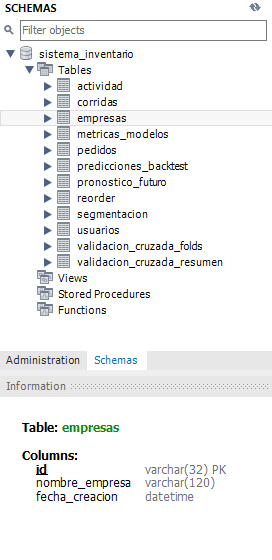
\includegraphics[height=0.35\textheight]{templatefigures/mysql_workbench_empresas}
    \caption{Estructura de la tabla \texttt{empresas} vista desde MySQL Workbench, conectado a la base de datos local.}
    \label{fig:mysql_workbench_empresas}
\end{figure}

La tabla \texttt{empresas} existe en la base de datos con las columnas descritas anteriormente: un identificador de tipo \texttt{varchar(32)} como clave primaria, el nombre de la empresa, y la fecha de creacion del registro.

\begin{figure}[H]
    \centering
    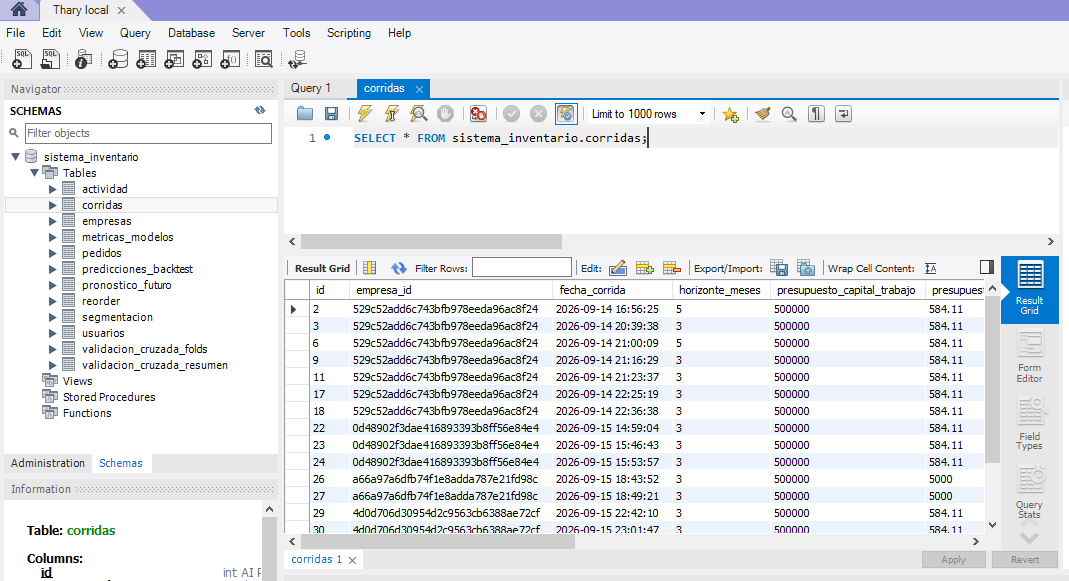
\includegraphics[height=0.3\textheight]{templatefigures/mysql_workbench_corridas}
    \caption{Consulta sobre la tabla \texttt{corridas} en MySQL Workbench, mostrando el esquema completo de 12 tablas y el historial acumulado de corridas.}
    \label{fig:mysql_workbench_corridas}
\end{figure}

La Fig. \ref{fig:mysql_workbench_corridas} muestra la confirmacion de que cada procesamiento de archivo genera una fila nueva en \texttt{corridas} sin eliminar las anteriores. Existen multiples filas asociadas a una misma empresa, correspondientes a distintas corridas realizadas en distintasfechas y horas.
